\section{Motivation}
\label{sec:motivation}

In Figure \ref{fig:motiv}, we illustrate an example from the Stack Overflow  \footnote{\small \url{https://stackoverflow.com/questions/55775450/}}.
\begin{figure}[h]
	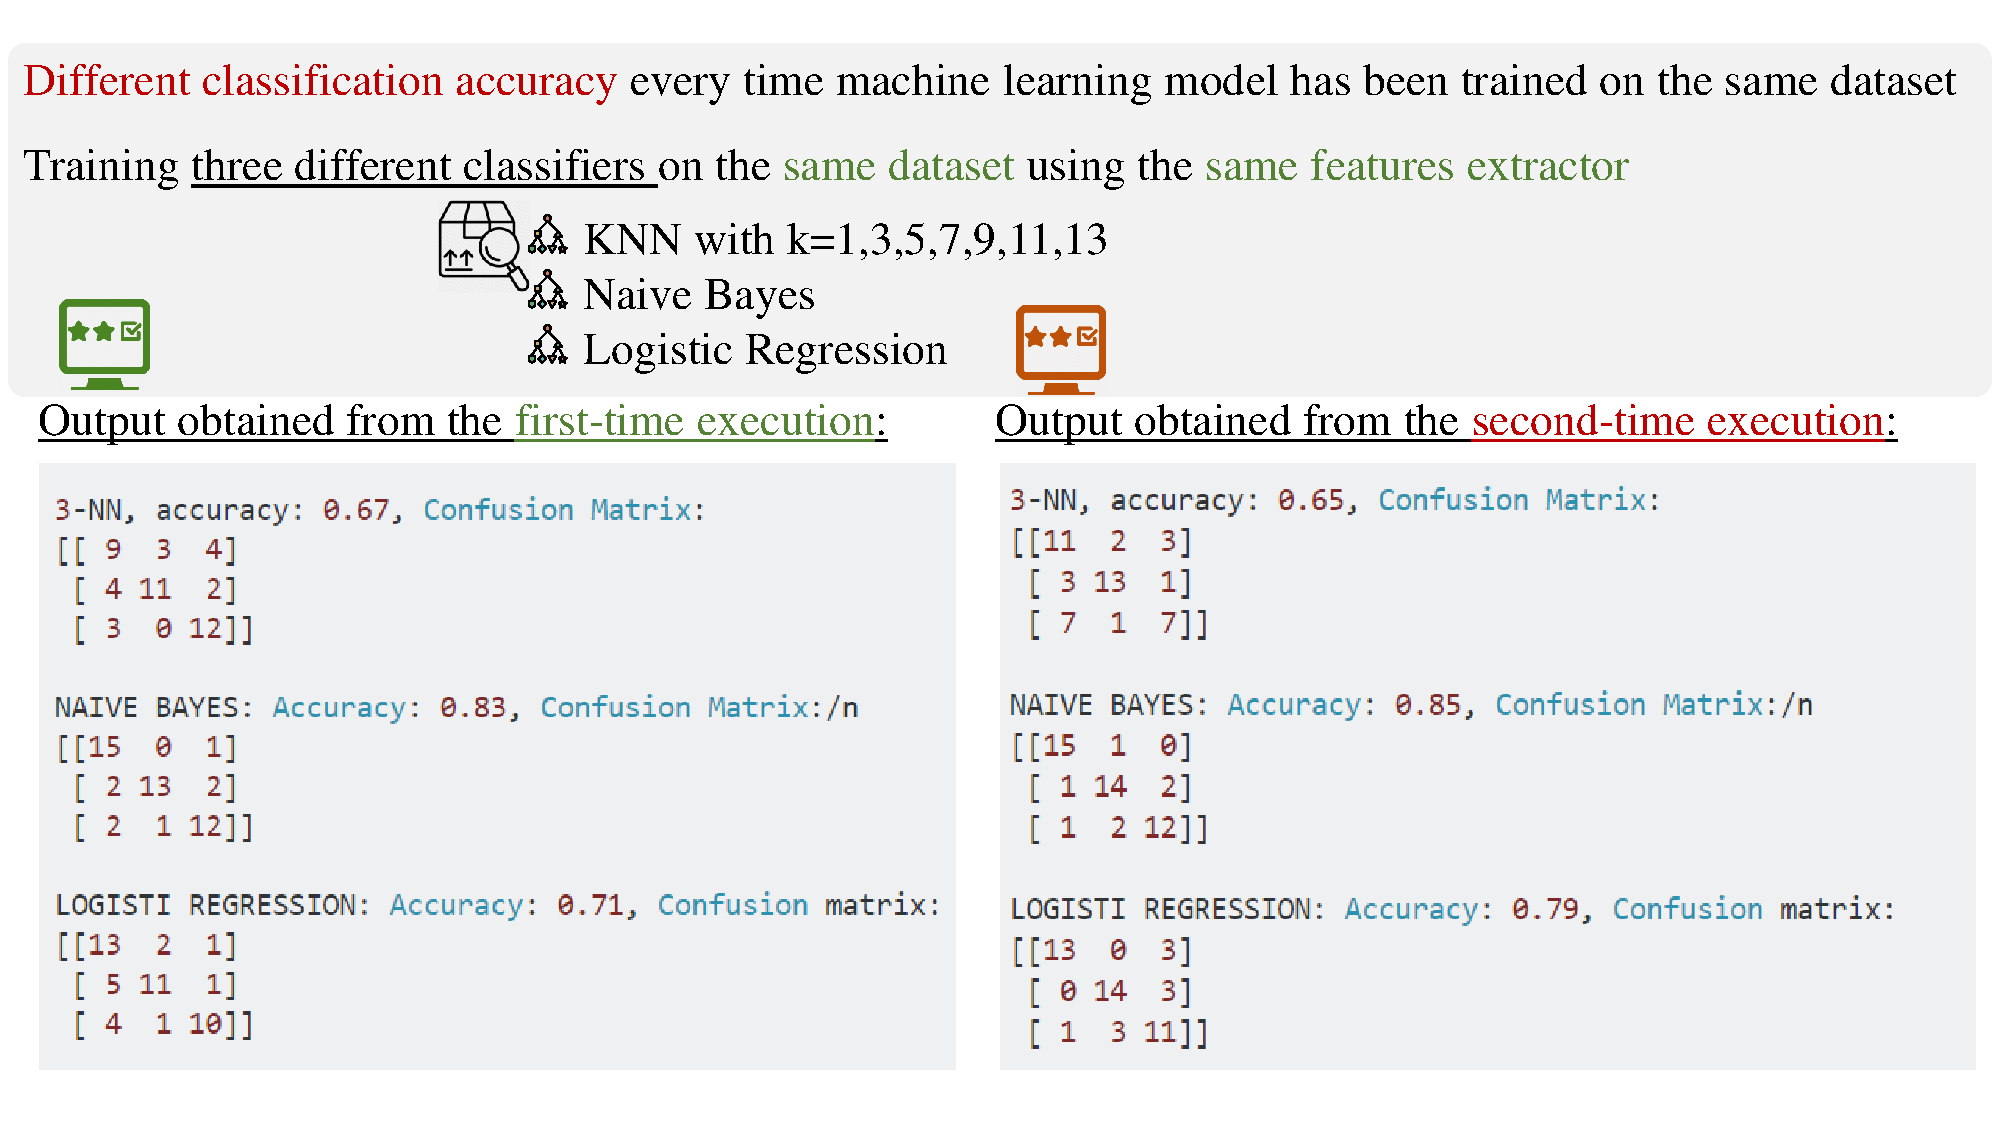
\includegraphics[width=\linewidth]{motivfigure.pdf}
	\caption{Example of different accuracy on each execution using same experimental setup}
	\label{fig:motiv}
	%\vspace{15pt}
\end{figure}

In this scenario, different classification accuracy has been obtained with every execution of a machine learning model that has been trained on the same dataset. Three different classifiers e.g., k-nearest neighbors, Naive Bayes, and Logistic Regression have been compared using the accuracy of each model. With every execution, these models have been trained with the same experimental setup, different values of accuracy for each model have been obtained as illustrated in Figure \ref{fig:motiv}. These results in a lack of trustworthiness of an ML-based model. The obvious question would be how we can interpret the accuracy or how the classifier can become accountable with the evaluation metric? This problem motivates us to propose a search-based approach and specification-based language to hold an DNN model accountable.  

%\small
%\begin{lstlisting}[language=Python, caption=Motivating example of model verification to interpret accuracy for accountable ML]
%//The first time execution of a CNN code gives this output:
%3-NN, accuracy: 0.67, Confusion Matrix:
%[[ 9  3  4]
%[ 4 11  2]
%[ 3  0 12]]
%
%NAIVE BAYES: Accuracy: 0.83, Confusion Matrix:/n
%[[15  0  1]
%[ 2 13  2]
%[ 2  1 12]]
%
%LOGISTIC REGRESSION: Accuracy: 0.71, Confusion matrix:
%[[13  2  1]
%[ 5 11  1]
%[ 4  1 10]]
%
%\\ The second time execution of the same code returns:
%3-NN, accuracy: 0.65, Confusion Matrix:
%[[11  2  3]
%[ 3 13  1]
%[ 7  1  7]]
%
%NAIVE BAYES: Accuracy: 0.85, Confusion Matrix:/n
%[[15  1  0]
%[ 1 14  2]
%[ 1  2 12]]
%
%LOGISTIC REGRESSION: Accuracy: 0.79, Confusion matrix:
%[[13  0  3]
%[ 0 14  3]
%[ 1  3 11]]
%\end{lstlisting}
